% Options for packages loaded elsewhere
\PassOptionsToPackage{unicode}{hyperref}
\PassOptionsToPackage{hyphens}{url}
\PassOptionsToPackage{dvipsnames,svgnames,x11names}{xcolor}
%
\documentclass[
  letterpaper,
  DIV=11,
  numbers=noendperiod]{scrartcl}

\usepackage{amsmath,amssymb}
\usepackage{lmodern}
\usepackage{iftex}
\ifPDFTeX
  \usepackage[T1]{fontenc}
  \usepackage[utf8]{inputenc}
  \usepackage{textcomp} % provide euro and other symbols
\else % if luatex or xetex
  \usepackage{unicode-math}
  \defaultfontfeatures{Scale=MatchLowercase}
  \defaultfontfeatures[\rmfamily]{Ligatures=TeX,Scale=1}
\fi
% Use upquote if available, for straight quotes in verbatim environments
\IfFileExists{upquote.sty}{\usepackage{upquote}}{}
\IfFileExists{microtype.sty}{% use microtype if available
  \usepackage[]{microtype}
  \UseMicrotypeSet[protrusion]{basicmath} % disable protrusion for tt fonts
}{}
\makeatletter
\@ifundefined{KOMAClassName}{% if non-KOMA class
  \IfFileExists{parskip.sty}{%
    \usepackage{parskip}
  }{% else
    \setlength{\parindent}{0pt}
    \setlength{\parskip}{6pt plus 2pt minus 1pt}}
}{% if KOMA class
  \KOMAoptions{parskip=half}}
\makeatother
\usepackage{xcolor}
\setlength{\emergencystretch}{3em} % prevent overfull lines
\setcounter{secnumdepth}{-\maxdimen} % remove section numbering
% Make \paragraph and \subparagraph free-standing
\ifx\paragraph\undefined\else
  \let\oldparagraph\paragraph
  \renewcommand{\paragraph}[1]{\oldparagraph{#1}\mbox{}}
\fi
\ifx\subparagraph\undefined\else
  \let\oldsubparagraph\subparagraph
  \renewcommand{\subparagraph}[1]{\oldsubparagraph{#1}\mbox{}}
\fi

\usepackage{color}
\usepackage{fancyvrb}
\newcommand{\VerbBar}{|}
\newcommand{\VERB}{\Verb[commandchars=\\\{\}]}
\DefineVerbatimEnvironment{Highlighting}{Verbatim}{commandchars=\\\{\}}
% Add ',fontsize=\small' for more characters per line
\usepackage{framed}
\definecolor{shadecolor}{RGB}{241,243,245}
\newenvironment{Shaded}{\begin{snugshade}}{\end{snugshade}}
\newcommand{\AlertTok}[1]{\textcolor[rgb]{0.68,0.00,0.00}{#1}}
\newcommand{\AnnotationTok}[1]{\textcolor[rgb]{0.37,0.37,0.37}{#1}}
\newcommand{\AttributeTok}[1]{\textcolor[rgb]{0.40,0.45,0.13}{#1}}
\newcommand{\BaseNTok}[1]{\textcolor[rgb]{0.68,0.00,0.00}{#1}}
\newcommand{\BuiltInTok}[1]{\textcolor[rgb]{0.00,0.23,0.31}{#1}}
\newcommand{\CharTok}[1]{\textcolor[rgb]{0.13,0.47,0.30}{#1}}
\newcommand{\CommentTok}[1]{\textcolor[rgb]{0.37,0.37,0.37}{#1}}
\newcommand{\CommentVarTok}[1]{\textcolor[rgb]{0.37,0.37,0.37}{\textit{#1}}}
\newcommand{\ConstantTok}[1]{\textcolor[rgb]{0.56,0.35,0.01}{#1}}
\newcommand{\ControlFlowTok}[1]{\textcolor[rgb]{0.00,0.23,0.31}{#1}}
\newcommand{\DataTypeTok}[1]{\textcolor[rgb]{0.68,0.00,0.00}{#1}}
\newcommand{\DecValTok}[1]{\textcolor[rgb]{0.68,0.00,0.00}{#1}}
\newcommand{\DocumentationTok}[1]{\textcolor[rgb]{0.37,0.37,0.37}{\textit{#1}}}
\newcommand{\ErrorTok}[1]{\textcolor[rgb]{0.68,0.00,0.00}{#1}}
\newcommand{\ExtensionTok}[1]{\textcolor[rgb]{0.00,0.23,0.31}{#1}}
\newcommand{\FloatTok}[1]{\textcolor[rgb]{0.68,0.00,0.00}{#1}}
\newcommand{\FunctionTok}[1]{\textcolor[rgb]{0.28,0.35,0.67}{#1}}
\newcommand{\ImportTok}[1]{\textcolor[rgb]{0.00,0.46,0.62}{#1}}
\newcommand{\InformationTok}[1]{\textcolor[rgb]{0.37,0.37,0.37}{#1}}
\newcommand{\KeywordTok}[1]{\textcolor[rgb]{0.00,0.23,0.31}{#1}}
\newcommand{\NormalTok}[1]{\textcolor[rgb]{0.00,0.23,0.31}{#1}}
\newcommand{\OperatorTok}[1]{\textcolor[rgb]{0.37,0.37,0.37}{#1}}
\newcommand{\OtherTok}[1]{\textcolor[rgb]{0.00,0.23,0.31}{#1}}
\newcommand{\PreprocessorTok}[1]{\textcolor[rgb]{0.68,0.00,0.00}{#1}}
\newcommand{\RegionMarkerTok}[1]{\textcolor[rgb]{0.00,0.23,0.31}{#1}}
\newcommand{\SpecialCharTok}[1]{\textcolor[rgb]{0.37,0.37,0.37}{#1}}
\newcommand{\SpecialStringTok}[1]{\textcolor[rgb]{0.13,0.47,0.30}{#1}}
\newcommand{\StringTok}[1]{\textcolor[rgb]{0.13,0.47,0.30}{#1}}
\newcommand{\VariableTok}[1]{\textcolor[rgb]{0.07,0.07,0.07}{#1}}
\newcommand{\VerbatimStringTok}[1]{\textcolor[rgb]{0.13,0.47,0.30}{#1}}
\newcommand{\WarningTok}[1]{\textcolor[rgb]{0.37,0.37,0.37}{\textit{#1}}}

\providecommand{\tightlist}{%
  \setlength{\itemsep}{0pt}\setlength{\parskip}{0pt}}\usepackage{longtable,booktabs,array}
\usepackage{calc} % for calculating minipage widths
% Correct order of tables after \paragraph or \subparagraph
\usepackage{etoolbox}
\makeatletter
\patchcmd\longtable{\par}{\if@noskipsec\mbox{}\fi\par}{}{}
\makeatother
% Allow footnotes in longtable head/foot
\IfFileExists{footnotehyper.sty}{\usepackage{footnotehyper}}{\usepackage{footnote}}
\makesavenoteenv{longtable}
\usepackage{graphicx}
\makeatletter
\def\maxwidth{\ifdim\Gin@nat@width>\linewidth\linewidth\else\Gin@nat@width\fi}
\def\maxheight{\ifdim\Gin@nat@height>\textheight\textheight\else\Gin@nat@height\fi}
\makeatother
% Scale images if necessary, so that they will not overflow the page
% margins by default, and it is still possible to overwrite the defaults
% using explicit options in \includegraphics[width, height, ...]{}
\setkeys{Gin}{width=\maxwidth,height=\maxheight,keepaspectratio}
% Set default figure placement to htbp
\makeatletter
\def\fps@figure{htbp}
\makeatother

\usepackage{fontspec}
\usepackage{multirow}
\usepackage{multicol}
\usepackage{colortbl}
\usepackage{hhline}
\newlength\Oldarrayrulewidth
\newlength\Oldtabcolsep
\usepackage{longtable}
\usepackage{array}
\usepackage{hyperref}
\usepackage{float}
\usepackage{wrapfig}
\KOMAoption{captions}{tableheading}
\makeatletter
\makeatother
\makeatletter
\makeatother
\makeatletter
\@ifpackageloaded{caption}{}{\usepackage{caption}}
\AtBeginDocument{%
\ifdefined\contentsname
  \renewcommand*\contentsname{Table of contents}
\else
  \newcommand\contentsname{Table of contents}
\fi
\ifdefined\listfigurename
  \renewcommand*\listfigurename{List of Figures}
\else
  \newcommand\listfigurename{List of Figures}
\fi
\ifdefined\listtablename
  \renewcommand*\listtablename{List of Tables}
\else
  \newcommand\listtablename{List of Tables}
\fi
\ifdefined\figurename
  \renewcommand*\figurename{Figure}
\else
  \newcommand\figurename{Figure}
\fi
\ifdefined\tablename
  \renewcommand*\tablename{Table}
\else
  \newcommand\tablename{Table}
\fi
}
\@ifpackageloaded{float}{}{\usepackage{float}}
\floatstyle{ruled}
\@ifundefined{c@chapter}{\newfloat{codelisting}{h}{lop}}{\newfloat{codelisting}{h}{lop}[chapter]}
\floatname{codelisting}{Listing}
\newcommand*\listoflistings{\listof{codelisting}{List of Listings}}
\makeatother
\makeatletter
\@ifpackageloaded{caption}{}{\usepackage{caption}}
\@ifpackageloaded{subcaption}{}{\usepackage{subcaption}}
\makeatother
\makeatletter
\@ifpackageloaded{tcolorbox}{}{\usepackage[many]{tcolorbox}}
\makeatother
\makeatletter
\@ifundefined{shadecolor}{\definecolor{shadecolor}{rgb}{.97, .97, .97}}
\makeatother
\makeatletter
\makeatother
\ifLuaTeX
  \usepackage{selnolig}  % disable illegal ligatures
\fi
\IfFileExists{bookmark.sty}{\usepackage{bookmark}}{\usepackage{hyperref}}
\IfFileExists{xurl.sty}{\usepackage{xurl}}{} % add URL line breaks if available
\urlstyle{same} % disable monospaced font for URLs
\hypersetup{
  pdftitle={ENVS 193DS Homework 4},
  pdfauthor={Lauren Stiles},
  colorlinks=true,
  linkcolor={blue},
  filecolor={Maroon},
  citecolor={Blue},
  urlcolor={Blue},
  pdfcreator={LaTeX via pandoc}}

\title{ENVS 193DS Homework 4}
\author{Lauren Stiles}
\date{}

\begin{document}
\maketitle
\ifdefined\Shaded\renewenvironment{Shaded}{\begin{tcolorbox}[sharp corners, frame hidden, enhanced, borderline west={3pt}{0pt}{shadecolor}, boxrule=0pt, interior hidden, breakable]}{\end{tcolorbox}}\fi

\textbf{Problem 1. How does fish length predict fish weight for trout
perch (across all sample years)?} 1. The null hypothesis is that the
predictor variable does not predict the response variable, or that the
fish length does not predict fish weight for trout perch. The
alternative hypothesis is that the the predictor variable does predict
the response variable, or that the fish length does predict fish weight
for trout perch.

\#Read in data and filter for desired variables

\begin{Shaded}
\begin{Highlighting}[]
\FunctionTok{library}\NormalTok{(tidyverse)}
\FunctionTok{library}\NormalTok{(here) }
\FunctionTok{library}\NormalTok{(naniar)}
\FunctionTok{library}\NormalTok{(performance)}
\FunctionTok{library}\NormalTok{(broom) }\CommentTok{\#puts all outputs from model into a table}
\FunctionTok{library}\NormalTok{(flextable) }\CommentTok{\#whole manual online, allows you to create tables that render nicely }
\FunctionTok{library}\NormalTok{(ggeffects) }\CommentTok{\#get predictions from models and plot them...}
\FunctionTok{library}\NormalTok{(car) }\CommentTok{\#pull out ANOVA tables specifically for linear models }


\CommentTok{\#read in data }
\NormalTok{fish\_dat }\OtherTok{\textless{}{-}} \FunctionTok{read\_csv}\NormalTok{(}\FunctionTok{here}\NormalTok{(}\StringTok{"data/ntl6\_v12.csv"}\NormalTok{))}

\CommentTok{\#filter out trout perch, select length and weight}
\NormalTok{trout\_dat }\OtherTok{\textless{}{-}}\NormalTok{ fish\_dat }\SpecialCharTok{|\textgreater{}} 
             \FunctionTok{mutate\_all}\NormalTok{(tolower)}\SpecialCharTok{|\textgreater{}} 
             \FunctionTok{filter}\NormalTok{(spname }\SpecialCharTok{==} \StringTok{"troutperch"}\NormalTok{) }\SpecialCharTok{|\textgreater{}} 
\NormalTok{             dplyr}\SpecialCharTok{::}\FunctionTok{select}\NormalTok{(length, weight) }\SpecialCharTok{|\textgreater{}} 
             \FunctionTok{mutate\_at}\NormalTok{(}\DecValTok{1}\SpecialCharTok{:}\DecValTok{2}\NormalTok{, as.numeric)}
\end{Highlighting}
\end{Shaded}

\begin{enumerate}
\def\labelenumi{\arabic{enumi}.}
\setcounter{enumi}{1}
\tightlist
\item
  Show missing data
\end{enumerate}

\begin{enumerate}
\def\labelenumi{\alph{enumi}.}
\tightlist
\item
\end{enumerate}

\begin{Shaded}
\begin{Highlighting}[]
\CommentTok{\#create visualization of missing data }
\NormalTok{missing\_data }\OtherTok{\textless{}{-}} \FunctionTok{gg\_miss\_var}\NormalTok{(trout\_dat) }\SpecialCharTok{+}
        \CommentTok{\#add caption}
        \FunctionTok{labs}\NormalTok{(}\AttributeTok{caption =} \StringTok{"Missing data in weight column might mean that test does not accurately represent how trout length predicts trout weight "}\NormalTok{) }\SpecialCharTok{+} 
        \FunctionTok{theme}\NormalTok{(}\CommentTok{\#change size of plot title }
        \AttributeTok{plot.title =} \FunctionTok{element\_text}\NormalTok{(}\AttributeTok{size =} \DecValTok{15}\NormalTok{),}
        \CommentTok{\#change size and location of plot caption}
        \AttributeTok{plot.caption =} \FunctionTok{element\_text}\NormalTok{(}\AttributeTok{size =} \FloatTok{6.5}\NormalTok{, }\AttributeTok{hjust =} \DecValTok{0}\NormalTok{),}
        \CommentTok{\#choose margins of plot }
        \AttributeTok{plot.margin =} \FunctionTok{unit}\NormalTok{(}\FunctionTok{c}\NormalTok{(}\DecValTok{1}\NormalTok{,}\DecValTok{1}\NormalTok{,}\DecValTok{1}\NormalTok{,}\DecValTok{1}\NormalTok{), }\StringTok{"cm"}\NormalTok{),}
        \CommentTok{\#change axis title size}
        \AttributeTok{axis.title =} \FunctionTok{element\_text}\NormalTok{(}\AttributeTok{size =} \DecValTok{12}\NormalTok{), }
        \CommentTok{\#change axis text size }
        \AttributeTok{axis.text =} \FunctionTok{element\_text}\NormalTok{(}\AttributeTok{size =} \DecValTok{10}\NormalTok{),}
        \CommentTok{\#remove axis ticks }
        \AttributeTok{axis.ticks =} \FunctionTok{element\_blank}\NormalTok{())}
      


\NormalTok{missing\_data}
\end{Highlighting}
\end{Shaded}

\begin{figure}[H]

{\centering 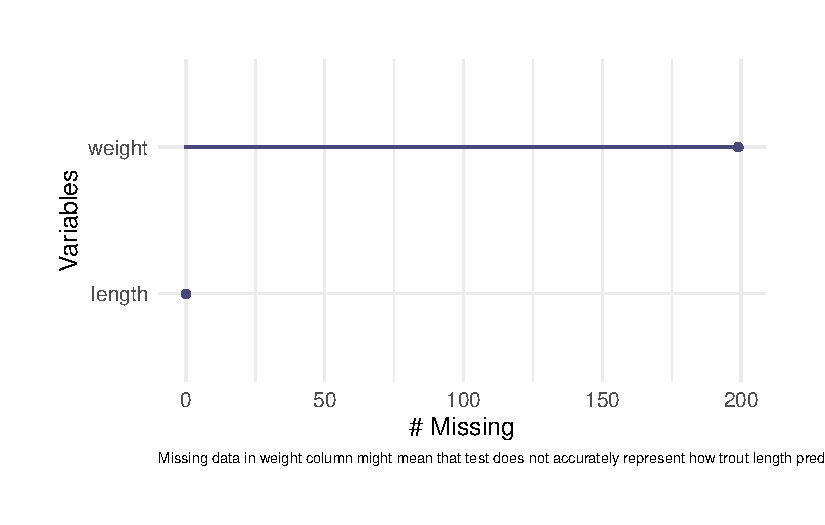
\includegraphics{ENVS-193DS-Homework-4_files/figure-pdf/unnamed-chunk-2-1.pdf}

}

\end{figure}

\begin{enumerate}
\def\labelenumi{\arabic{enumi}.}
\setcounter{enumi}{2}
\tightlist
\item
  Running test
\end{enumerate}

\begin{Shaded}
\begin{Highlighting}[]
\CommentTok{\#run linear model looking into relationship between length and weight}
\NormalTok{trout\_model }\OtherTok{\textless{}{-}} \FunctionTok{lm}\NormalTok{(weight }\SpecialCharTok{\textasciitilde{}}\NormalTok{ length, }\AttributeTok{data =}\NormalTok{ trout\_dat)}
\NormalTok{trout\_model}
\end{Highlighting}
\end{Shaded}

\begin{verbatim}

Call:
lm(formula = weight ~ length, data = trout_dat)

Coefficients:
(Intercept)       length  
   -11.7025       0.1999  
\end{verbatim}

\begin{enumerate}
\def\labelenumi{\arabic{enumi}.}
\setcounter{enumi}{3}
\tightlist
\item
  Visually check test assumptions
\end{enumerate}

\begin{Shaded}
\begin{Highlighting}[]
\FunctionTok{par}\NormalTok{(}\AttributeTok{mfrow =} \FunctionTok{c}\NormalTok{(}\DecValTok{2}\NormalTok{,}\DecValTok{2}\NormalTok{))}
\FunctionTok{plot}\NormalTok{(trout\_model)}
\end{Highlighting}
\end{Shaded}

\begin{figure}[H]

{\centering 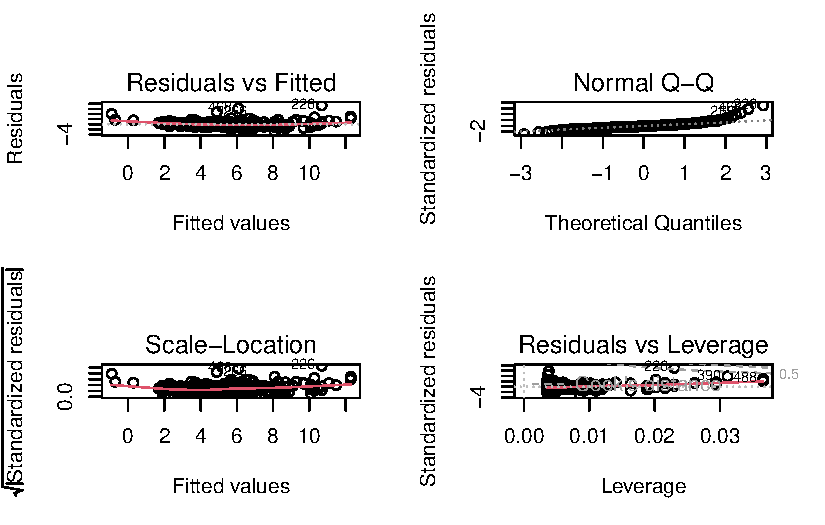
\includegraphics{ENVS-193DS-Homework-4_files/figure-pdf/unnamed-chunk-4-1.pdf}

}

\end{figure}

\begin{enumerate}
\def\labelenumi{\arabic{enumi}.}
\setcounter{enumi}{4}
\item
  The residuals versus fitted plot shows the distributions of residuals
  and a straight line indicates homoskedasticity, or constant variance
  of residuals. This plot looks homoskedastic to me since the line is
  relatively straight and the points look randomly distributed around
  the line. The normal q-q plot shows whether the residuals are normally
  distributed. Since the points appear to be in a mostly straight line,
  I would say that the residuals have a normal distribution. The
  scale-location plot also shows homoskedasticity of variance, but using
  the square root of the standardized residuals. They are in a somewhat
  straight line and the points seem randomly distributed about it, so
  they are homoskedastic.The residuals vs leverage, or the cook's
  distance plot shows whether outliers are influencing the model
  estimate. There are some that are labeled as outliers, but only one
  outside the dotted line range, so it does not appear that there are
  outliers significantly affecting model predictions.
\item
\end{enumerate}

\begin{Shaded}
\begin{Highlighting}[]
\CommentTok{\#run a summary of the model object }
\FunctionTok{summary}\NormalTok{(trout\_model)}
\end{Highlighting}
\end{Shaded}

\begin{verbatim}

Call:
lm(formula = weight ~ length, data = trout_dat)

Residuals:
    Min      1Q  Median      3Q     Max 
-3.0828 -0.4862 -0.1830  0.4128  7.3191 

Coefficients:
              Estimate Std. Error t value Pr(>|t|)    
(Intercept) -11.702476   0.481564  -24.30   <2e-16 ***
length        0.199852   0.005584   35.79   <2e-16 ***
---
Signif. codes:  0 '***' 0.001 '**' 0.01 '*' 0.05 '.' 0.1 ' ' 1

Residual standard error: 1.057 on 288 degrees of freedom
  (199 observations deleted due to missingness)
Multiple R-squared:  0.8164,    Adjusted R-squared:  0.8158 
F-statistic:  1281 on 1 and 288 DF,  p-value: < 2.2e-16
\end{verbatim}

\begin{enumerate}
\def\labelenumi{\arabic{enumi}.}
\setcounter{enumi}{6}
\tightlist
\item
\end{enumerate}

\begin{Shaded}
\begin{Highlighting}[]
\CommentTok{\#make table showing ANOVA table summary }
\NormalTok{trout\_model\_squares }\OtherTok{\textless{}{-}} \FunctionTok{anova}\NormalTok{(trout\_model)}


\NormalTok{trout\_model\_squares\_table }\OtherTok{\textless{}{-}} \FunctionTok{tidy}\NormalTok{(trout\_model\_squares) }\SpecialCharTok{|\textgreater{}} 
                       \FunctionTok{mutate}\NormalTok{(}\AttributeTok{p.value =} \FunctionTok{case\_when}\NormalTok{(p.value }\SpecialCharTok{\textless{}}\FloatTok{0.001} \SpecialCharTok{\textasciitilde{}} \StringTok{"\textless{} 0.001"}\NormalTok{)) }\SpecialCharTok{|\textgreater{}}
                       \FunctionTok{flextable}\NormalTok{() }\SpecialCharTok{|\textgreater{}}  \CommentTok{\#easiest way to make this into a table }
                       \FunctionTok{set\_header\_labels}\NormalTok{(}\AttributeTok{df =} \StringTok{"Degrees of Freedom"}\NormalTok{, }\AttributeTok{sumsq =} \StringTok{"Sum of Squares"}\NormalTok{,                        }\AttributeTok{meansq =} \StringTok{"Mean squares"}\NormalTok{, }\AttributeTok{statistic =} \StringTok{"F{-}statistic"}\NormalTok{)}

\NormalTok{trout\_model\_squares\_table}
\end{Highlighting}
\end{Shaded}

\global\setlength{\Oldarrayrulewidth}{\arrayrulewidth}

\global\setlength{\Oldtabcolsep}{\tabcolsep}

\setlength{\tabcolsep}{0pt}

\renewcommand*{\arraystretch}{1.5}



\providecommand{\ascline}[3]{\noalign{\global\arrayrulewidth #1}\arrayrulecolor[HTML]{#2}\cline{#3}}

\begin{longtable}[c]{|p{0.75in}|p{0.75in}|p{0.75in}|p{0.75in}|p{0.75in}|p{0.75in}}



\ascline{1.5pt}{666666}{1-6}

\multicolumn{1}{>{\raggedright}m{\dimexpr 0.75in+0\tabcolsep}}{\textcolor[HTML]{000000}{\fontsize{11}{11}\selectfont{term}}} & \multicolumn{1}{>{\raggedleft}m{\dimexpr 0.75in+0\tabcolsep}}{\textcolor[HTML]{000000}{\fontsize{11}{11}\selectfont{Degrees\ of\ Freedom}}} & \multicolumn{1}{>{\raggedleft}m{\dimexpr 0.75in+0\tabcolsep}}{\textcolor[HTML]{000000}{\fontsize{11}{11}\selectfont{Sum\ of\ Squares}}} & \multicolumn{1}{>{\raggedleft}m{\dimexpr 0.75in+0\tabcolsep}}{\textcolor[HTML]{000000}{\fontsize{11}{11}\selectfont{Mean\ squares}}} & \multicolumn{1}{>{\raggedleft}m{\dimexpr 0.75in+0\tabcolsep}}{\textcolor[HTML]{000000}{\fontsize{11}{11}\selectfont{F-statistic}}} & \multicolumn{1}{>{\raggedright}m{\dimexpr 0.75in+0\tabcolsep}}{\textcolor[HTML]{000000}{\fontsize{11}{11}\selectfont{p.value}}} \\

\ascline{1.5pt}{666666}{1-6}\endhead



\multicolumn{1}{>{\raggedright}m{\dimexpr 0.75in+0\tabcolsep}}{\textcolor[HTML]{000000}{\fontsize{11}{11}\selectfont{length}}} & \multicolumn{1}{>{\raggedleft}m{\dimexpr 0.75in+0\tabcolsep}}{\textcolor[HTML]{000000}{\fontsize{11}{11}\selectfont{1}}} & \multicolumn{1}{>{\raggedleft}m{\dimexpr 0.75in+0\tabcolsep}}{\textcolor[HTML]{000000}{\fontsize{11}{11}\selectfont{1,432.2877}}} & \multicolumn{1}{>{\raggedleft}m{\dimexpr 0.75in+0\tabcolsep}}{\textcolor[HTML]{000000}{\fontsize{11}{11}\selectfont{1,432.287687}}} & \multicolumn{1}{>{\raggedleft}m{\dimexpr 0.75in+0\tabcolsep}}{\textcolor[HTML]{000000}{\fontsize{11}{11}\selectfont{1,280.844}}} & \multicolumn{1}{>{\raggedright}m{\dimexpr 0.75in+0\tabcolsep}}{\textcolor[HTML]{000000}{\fontsize{11}{11}\selectfont{<\ 0.001}}} \\





\multicolumn{1}{>{\raggedright}m{\dimexpr 0.75in+0\tabcolsep}}{\textcolor[HTML]{000000}{\fontsize{11}{11}\selectfont{Residuals}}} & \multicolumn{1}{>{\raggedleft}m{\dimexpr 0.75in+0\tabcolsep}}{\textcolor[HTML]{000000}{\fontsize{11}{11}\selectfont{288}}} & \multicolumn{1}{>{\raggedleft}m{\dimexpr 0.75in+0\tabcolsep}}{\textcolor[HTML]{000000}{\fontsize{11}{11}\selectfont{322.0525}}} & \multicolumn{1}{>{\raggedleft}m{\dimexpr 0.75in+0\tabcolsep}}{\textcolor[HTML]{000000}{\fontsize{11}{11}\selectfont{1.118238}}} & \multicolumn{1}{>{\raggedleft}m{\dimexpr 0.75in+0\tabcolsep}}{\textcolor[HTML]{000000}{\fontsize{11}{11}\selectfont{}}} & \multicolumn{1}{>{\raggedright}m{\dimexpr 0.75in+0\tabcolsep}}{\textcolor[HTML]{000000}{\fontsize{11}{11}\selectfont{}}} \\

\ascline{1.5pt}{666666}{1-6}



\end{longtable}



\arrayrulecolor[HTML]{000000}

\global\setlength{\arrayrulewidth}{\Oldarrayrulewidth}

\global\setlength{\tabcolsep}{\Oldtabcolsep}

\renewcommand*{\arraystretch}{1}

\begin{enumerate}
\def\labelenumi{\arabic{enumi}.}
\setcounter{enumi}{7}
\item
  The ANOVA test is built on the same parametric base as linear
  regression models, so they have similar math and outputs.The ANOVA
  highlights some of the summary elements from the model object, giving
  more details about the test. ????
\item
  We can reject the null hypothesis since the linear regression model
  summary resulted in a p-value of \textless0.001. Based on our
  observations, we can expect a 0.2g increase in fish weight as fish
  length (mm) increases, as shown by the linear model() (F{[}1,288{]} =
  )
\item
  Prediction Visualization
\end{enumerate}

\begin{Shaded}
\begin{Highlighting}[]
\CommentTok{\#pulling out predictions}
\CommentTok{\#terms corresponds to whatever the predictor was in the model }
\NormalTok{predictions }\OtherTok{\textless{}{-}} \FunctionTok{ggpredict}\NormalTok{(trout\_model, }\AttributeTok{terms =} \StringTok{"length"}\NormalTok{)}

\CommentTok{\#plot predictions }
\NormalTok{plot\_predictions }\OtherTok{\textless{}{-}} \FunctionTok{ggplot}\NormalTok{(}\AttributeTok{data =}\NormalTok{ trout\_dat, }\FunctionTok{aes}\NormalTok{(length, }\AttributeTok{y =}\NormalTok{ weight)) }\SpecialCharTok{+} 
  \CommentTok{\#first plot the underlying data }
  \FunctionTok{geom\_point}\NormalTok{() }\SpecialCharTok{+} 
  \CommentTok{\#plotting model predictions from the predictions object from ggeffects}
  \FunctionTok{geom\_line}\NormalTok{(}\AttributeTok{data =}\NormalTok{ predictions, }\FunctionTok{aes}\NormalTok{(}\AttributeTok{x =}\NormalTok{ x, }\AttributeTok{y =}\NormalTok{ predicted), }\AttributeTok{color =} \StringTok{"blue"}\NormalTok{, }\AttributeTok{linewidth =} \DecValTok{1}\NormalTok{) }\SpecialCharTok{+} 
  \CommentTok{\#plot the confidence interval around model estimates }
  \FunctionTok{geom\_ribbon}\NormalTok{(}\AttributeTok{data =}\NormalTok{ predictions, }\FunctionTok{aes}\NormalTok{(}\AttributeTok{x =}\NormalTok{ x, }\AttributeTok{y =}\NormalTok{ predicted, }\AttributeTok{ymin =}\NormalTok{ conf.low, }\AttributeTok{ymax =}\NormalTok{ conf.high), }\AttributeTok{alpha =} \FloatTok{0.2}\NormalTok{) }\SpecialCharTok{+} 
\CommentTok{\#do not use geom\_smooth because it does not tell you where the model comes from, what the equation is, standard intervals, ect...}
   \FunctionTok{labs}\NormalTok{(}\AttributeTok{x =} \StringTok{"Length"}\NormalTok{, }
        \AttributeTok{y =} \StringTok{"Weight"}\NormalTok{, }
        \AttributeTok{title =} \StringTok{"Trout Perch Weight Predicted by Length"}\NormalTok{, }
        \AttributeTok{caption =} \StringTok{"Figure 2. Dots show predicted values for fish weight based on size and the blue line shows the equation from the linear regression run on to test this prediction"}\NormalTok{) }\SpecialCharTok{+}
  \FunctionTok{theme\_bw}\NormalTok{() }\SpecialCharTok{+}
  \CommentTok{\#change text font}
  \FunctionTok{theme}\NormalTok{(}\CommentTok{\#change size of plot title }
        \AttributeTok{plot.title =} \FunctionTok{element\_text}\NormalTok{(}\AttributeTok{size =} \DecValTok{15}\NormalTok{),}
        \CommentTok{\#change size and location of plot caption}
        \AttributeTok{plot.caption =} \FunctionTok{element\_text}\NormalTok{(}\AttributeTok{size =} \FloatTok{6.5}\NormalTok{, }\AttributeTok{hjust =} \DecValTok{0}\NormalTok{),}
        \CommentTok{\#choose margins of plot }
        \AttributeTok{plot.margin =} \FunctionTok{unit}\NormalTok{(}\FunctionTok{c}\NormalTok{(}\DecValTok{1}\NormalTok{,}\DecValTok{1}\NormalTok{,}\DecValTok{1}\NormalTok{,}\DecValTok{1}\NormalTok{), }\StringTok{"cm"}\NormalTok{),}
        \CommentTok{\#change axis title size}
        \AttributeTok{axis.title =} \FunctionTok{element\_text}\NormalTok{(}\AttributeTok{size =} \DecValTok{12}\NormalTok{), }
        \CommentTok{\#change axis text size }
        \AttributeTok{axis.text =} \FunctionTok{element\_text}\NormalTok{(}\AttributeTok{size =} \DecValTok{10}\NormalTok{),}
        \CommentTok{\#remove axis ticks }
        \AttributeTok{axis.ticks =} \FunctionTok{element\_blank}\NormalTok{())}
      

\NormalTok{plot\_predictions}
\end{Highlighting}
\end{Shaded}

\begin{figure}[H]

{\centering 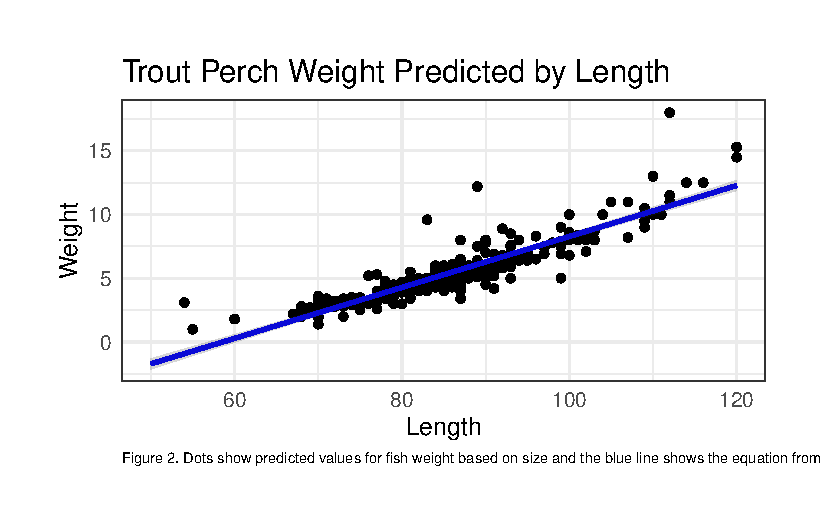
\includegraphics{ENVS-193DS-Homework-4_files/figure-pdf/unnamed-chunk-7-1.pdf}

}

\end{figure}



\end{document}
